% =====================================================================
% AJDSAI / AJEB submission - Asian Journal of Data Science and AI
% Style follows Emerald AJEB guidelines:
%   https://www.emeraldgrouppublishing.com/journal/ajeb
% =====================================================================
% Build: pdflatex main && bibtex main && pdflatex main && pdflatex main
% Or:    make
% =====================================================================

\documentclass[11pt, a4paper]{article}

% --- Page geometry: Emerald uses generous single-column margins ---
\usepackage[a4paper, top=2.5cm, bottom=2.5cm, left=2.5cm, right=2.5cm]{geometry}
\usepackage[T1]{fontenc}
\usepackage[utf8]{inputenc}
\usepackage{times}                  % Emerald house font is Times-like

% --- Spacing: Emerald uses 1.5 line spacing for submission ---
\usepackage{setspace}
\onehalfspacing

% --- Math, graphics, tables ---
\usepackage{graphicx}
\usepackage{amsmath, amssymb}
\usepackage{booktabs}
\usepackage{array}
\usepackage{multirow}
\usepackage{longtable}
\usepackage{tabularx}

% --- Hyperlinks (subtle for journal) ---
\usepackage[colorlinks=true, linkcolor=black, citecolor=black, urlcolor=blue]{hyperref}

% --- TikZ for pipeline diagram ---
\usepackage{tikz}
\usetikzlibrary{positioning, arrows.meta, shapes.geometric}

% --- Harvard citation style (Emerald house style) ---
\usepackage{natbib}
\bibliographystyle{agsm}            % Australian Govt. Style Manual = Emerald Harvard
\setcitestyle{authoryear, round}

% --- Section formatting: Emerald uses unnumbered sections in some styles,
%     but numbered is acceptable. We use numbered. ---
\usepackage{titlesec}
\titleformat{\section}{\bfseries\large}{\thesection.}{0.5em}{}
\titleformat{\subsection}{\bfseries\normalsize}{\thesubsection}{0.5em}{}

% --- Caption style ---
\usepackage[font=small, labelfont=bf]{caption}

% --- Figure placement ---
\usepackage{float}

\setlength{\parindent}{0pt}
\setlength{\parskip}{0.5em}

% =====================================================================
\begin{document}

% --- TITLE BLOCK (Emerald: title, then authors, then affiliations as numbered list) ---
\begin{center}
{\Large \textbf{Parameter-Efficient Quantum Sentiment Classification:\\
A Controlled Empirical Study of DisCoCat on SST-2}}

\vspace{1em}

{\large Nhat-Linh Do$^{1}$, Quang-Thai Le$^{1}$, Minh-Tan Tran-Huynh$^{2}$}

\vspace{0.6em}

\emph{$^{1}$Faculty of Business Data Science,
Banking University of Ho Chi Minh City, Vietnam}\\[0.2em]
\emph{$^{2}$Faculty of Management Information Systems,
Banking University of Ho Chi Minh City, Vietnam}

\vspace{0.4em}

\texttt{linh.do@hub.edu.vn, thailq@hub.edu.vn, tanthm@hub.edu.vn}

\vspace{1em}
\end{center}

% =====================================================================
% STRUCTURED ABSTRACT (Emerald mandatory format)
% =====================================================================

\noindent\textbf{Structured Abstract}

\vspace{0.5em}

\noindent\textbf{Purpose --- }
This study investigates the practical performance of Quantum Natural
Language Processing (QNLP) for binary sentiment classification, focusing
on whether variational quantum circuits built from Distributional
Compositional Categorical (DisCoCat) diagrams can attain accuracy
competitive with classical baselines on a public benchmark while using a
substantially smaller parameter budget.

\vspace{0.4em}

\noindent\textbf{Design/methodology/approach --- }
A controlled experimental grid of 60 quantum training runs is reported
on a class-balanced 5{,}000/400/400 subset of the Stanford Sentiment
Treebank. The grid spans two diagram readers (Spiders, Cups), two
ansatz families (IQP, Sim14), three circuit depths and five random
seeds. Three classical baselines---Logistic Regression with TF--IDF
bigrams, Logistic Regression with averaged GloVe embeddings, and a
single-layer bidirectional LSTM---are evaluated on the same data split.
Differences between models are assessed using paired McNemar tests.

\vspace{0.4em}

\noindent\textbf{Findings --- }
The Spiders reader (identical accuracy across all six ansatz--depth
configurations, as documented below) attains \(92.05\% \pm 0.64\%\)
test accuracy with only \(2{,}940\) trainable parameters, a result
that is statistically indistinguishable from the BiLSTM baseline
(\(91.83\% \pm 0.42\%\); McNemar \(p = 0.60\)) which requires \(28\)
times as many parameters, while trailing the sparse linear baseline
LR + TF--IDF (\(94.25\%\), \(2{,}829\) parameters; McNemar
\(p = 0.045\)) by a small but statistically detectable margin. Two
methodologically informative findings are reported: (i) with
single-qubit atomic types the Spiders reader is representationally
degenerate and all six ansatz/depth combinations yield identical
accuracy; (ii) the Cups + IQP family at depth two falls into a
reproducible barren plateau (\(62.8\%\) accuracy across all five
seeds) that persists under standard mitigation strategies.

\vspace{0.4em}

\noindent\textbf{Originality/value --- }
The paper contributes a reproducible end-to-end QNLP pipeline on a
public benchmark, a systematic 60-run ablation of reader \(\times\) ansatz \(\times\)
depth interactions for short-phrase sentiment, an empirical case study of the barren-plateau phenomenon in
applied QNLP, and a documentation of an infrastructure-level
reproducibility issue affecting the \texttt{lambeq} 0.5 BobcatParser
model distribution.

\vspace{0.4em}

\noindent\textbf{Practical implications --- }
For practitioners in finance and business analytics who are exploring
quantum machine learning, the results indicate that variational
quantum models can match a small classical neural baseline at
substantially lower parameter cost on short-text tasks. This has direct
relevance to customer-feedback analysis, social-media sentiment
extraction and product-review classification on resource-constrained
quantum simulators or near-term NISQ hardware.

\vspace{0.4em}

\noindent\textbf{Keywords:} Quantum Natural Language Processing,
DisCoCat, Variational Quantum Circuits, Sentiment Classification,
Barren Plateau, Parameter Efficiency

\vspace{0.4em}

\noindent\textbf{Paper type:} Research paper

\vspace{1.5em}

% =====================================================================
\section{Introduction}
\label{sec:intro}

Recent progress in Natural Language Processing (NLP) has been dominated
by large pretrained language models whose parameter counts run into the
hundreds of millions or billions. While the empirical performance of
these models is impressive, their resource requirements place them
well beyond the capabilities of current near-term quantum hardware.
Quantum Natural Language Processing (QNLP), formalised in the
Distributional Compositional Categorical (DisCoCat) framework of
\citet{coecke2010}, offers a structurally different approach in which
sentence meaning is built compositionally from word tensors according
to the pregroup grammar of the sentence. Because grammatical
composition maps naturally onto qubit registers and entangling gates,
DisCoCat models can be realised directly as variational quantum
circuits and trained on simulators or, in principle, on NISQ
hardware~\citep{lorenz2021, kartsaklis2021}.

We address three questions in this practical context.
How does a variational quantum DisCoCat model trained on a public
sentiment benchmark compare with classical baselines of comparable
size? Which design choices in the QNLP pipeline (reader, ansatz, or
circuit depth) are the primary drivers of performance? And how
reliably can such models be trained in practice given the well-known
optimisation pathologies of variational quantum
algorithms~\citep{mcclean2018}?

To answer these questions, a controlled experimental grid of 60
quantum training runs is conducted on a class-balanced
\(5{,}000/400/400\) subset of the Stanford Sentiment Treebank
\citep{socher2013}, spanning two readers, two ansatz families, three
circuit depths and five random seeds. Three classical baselines of
different inductive bias---Logistic Regression with TF--IDF bigrams,
Logistic Regression with averaged GloVe embeddings, and a
single-layer Bidirectional LSTM---are evaluated on the same split.

The contributions of the paper are threefold. First, a fully
reproducible pipeline from raw Stanford Sentiment Treebank data,
through DisCoCat diagrams and quantum circuits, to final evaluation
metrics is released as open source at
\url{https://github.com/hublinhdn/nlp_quantum_hub}, including all
preprocessing decisions, hyperparameters, evaluation procedures and
the per-seed prediction artefacts required to reproduce every figure
and table in this paper. Second, the 60-run grid produces
two methodologically informative observations: the Spiders reader with
single-qubit atomic types is representationally degenerate, and the
Cups + IQP family falls into a reproducible barren plateau at depth
two. Third, an infrastructure-level reproducibility issue is
documented (the deprecated \texttt{qnlp.cambridgequantum.com} domain
referenced by \texttt{lambeq} 0.5.0 for the BobcatParser model), and
a workaround based on the self-contained Spiders and Cups readers is
described.

The remainder of the paper is organised as follows.
Section~\ref{sec:related} reviews the DisCoCat framework, QNLP
literature and variational quantum circuit ansatzes.
Section~\ref{sec:method} describes the data pipeline, models and
training protocol. Section~\ref{sec:results} reports the main
experimental results. Section~\ref{sec:discussion} discusses
implications, limitations and practical considerations.
Section~\ref{sec:conclusion} concludes.

% =====================================================================
\section{Literature Review}
\label{sec:related}

\subsection{DisCoCat and Compositional Distributional Semantics}

The Distributional Compositional Categorical model
\citep{coecke2010} unifies two strands of computational semantics:
distributional word representations, in which words are vectors in a
high-dimensional space, and compositional grammar, in which sentences
are constructed by combining word meanings according to syntactic
structure. The framework uses pregroup grammar~\citep{lambek1958} to
assign each word a type formed from atomic categories (e.g.\ \(n\) for
noun, \(s\) for sentence) and their adjoints. A sentence is
grammatical if its sequence of types reduces to \(s\) under
contraction; the resulting reduction is represented as a string diagram
in a monoidal category, simultaneously encoding the syntactic
derivation and the semantic composition.

In the categorical formulation, words are morphisms from the
monoidal unit to a tensor product of atomic types, and the sentence is
the composition of those morphisms. Realising the composition in a
finite-dimensional Hilbert space therefore yields a direct mapping
between sentences and quantum states: words become parameterised
quantum states, atomic types become qubit registers, and grammatical
contractions are realised by measurement-induced post-selection or by
measurement of an output register.

\subsection{Quantum Natural Language Processing}

Practical QNLP toolchains have been developed by Quantinuum and
collaborators. The \texttt{lambeq} library~\citep{kartsaklis2021}
implements the full DisCoCat pipeline---CCG parsing, pregroup
conversion, rewriter application and ansatz functor, all in Python and
provides interfaces to multiple quantum back-ends, including PennyLane.
\citet{lorenz2021} demonstrate that small DisCoCat models can be
trained on real Quantinuum H1 hardware for binary classification of
~130 phrases, reaching accuracies in the region of \(80\%\).
\citet{meichanetzidis2020} provide complementary analysis on
near-term quantum devices. More recently, \citet{xu2024} introduce
quantum recurrent architectures for text classification at scale and
report results on standard NLP benchmarks. \citet{guarasci2024}
investigate quantum transfer learning for grammatical acceptability
judgements, demonstrating that QNLP models can transfer linguistic
knowledge across related tasks. Our work continues this line of
practical QNLP studies, but at order-of-magnitude larger scale than
\citet{lorenz2021} on a public benchmark, with five-seed statistical
analysis.

\subsection{Variational Quantum Ansatzes}

A variational quantum ansatz is a parameterised quantum circuit family
with fixed topology and trainable rotation angles. The IQP family
\citep{havlicek2019} alternates layers of single-qubit Hadamard gates
with diagonal phase entangling gates. The Sim14 family
\citep{sim2019}---one of nineteen circuit topologies catalogued by
\citet{sim2019}---uses controlled rotation gates in a hardware-efficient
pattern with strong per-layer entanglement. The number of layers
controls expressive capacity but also exposes the optimisation
landscape to the barren-plateau phenomenon
\citep{mcclean2018, cerezo2021}, in which gradient magnitudes vanish
exponentially with circuit size, rendering training intractable. The
training dynamics of these ansatzes on DisCoCat-derived circuits are
one of the central empirical questions in this paper.

\subsection{Sentiment Classification and the SST-2 Benchmark}

Sentiment classification is one of the most extensively studied tasks
in NLP and a canonical setting for evaluating new methods on short
text. Classical approaches range from sparse bag-of-words representations
combined with logistic regression \citep{scikit2011} through dense
distributed representations such as word2vec \citep{mikolov2013} and
GloVe \citep{pennington2014}, to sequential neural models including
LSTM-based architectures \citep{hochreiter1997} and, more recently,
transformer-based pretrained language models such as BERT
\citep{devlin2019bert}. Each family encodes a different inductive
bias: bag-of-words models capture lexical sentiment directly,
distributed embeddings encode semantic similarity in continuous
spaces, sequential models exploit token order, and transformer models
exploit large-scale pretraining. The QNLP framework, by contrast,
encodes \emph{compositional} structure directly into the model's
topology, an inductive bias that is, in principle, particularly
well-suited to phenomena such as negation, modification and
co-ordination.

The Stanford Sentiment Treebank \citep{socher2013} provides
fine-grained sentiment annotations on phrases extracted from parse
trees of movie reviews. The binary subset (SST-2), derived by
thresholding the continuous sentiment score, is one of the canonical
benchmarks for binary sentiment classification in classical NLP, and
forms part of the GLUE benchmark suite \citep{wang2018glue}. The
paper restricts attention to phrases of two to five tokens,
which is consistent with prior QNLP studies \citep{lorenz2021} and
keeps quantum simulation tractable on commodity hardware. The
restriction also matches the typical length of customer-feedback
fragments, product-review headers and microblog snippets that are
relevant to practical sentiment-analysis applications in finance and
business.

\subsection{Variational Quantum Algorithms and Optimisation Pathologies}

Variational quantum algorithms more generally have emerged as the
dominant paradigm for near-term quantum machine learning
\citep{cerezo2021, cerezo2022qml}. The training of these algorithms
is performed classically using gradient-based optimisation on a
parameterised quantum circuit \citep{mitarai2018, schuld2019}, with
the quantum device used only to evaluate expectation values. A line
of recent work, including \citet{schuld2022advantage}, has prompted a
more sober reassessment of whether quantum advantage is the right
benchmark for QML in the NISQ era, arguing that practical considerations
such as parameter efficiency and trainability may be more immediately
useful targets.

Among the most significant practical obstacles to variational quantum
training is the barren-plateau phenomenon \citep{mcclean2018},
in which the variance of gradients vanishes exponentially with the
number of qubits or circuit depth, rendering the loss landscape
effectively flat over wide parameter ranges. The theoretical
foundations of this phenomenon have been recently consolidated in the
review of \citet{larocca2025} and the Lie algebraic characterisation
of \citet{ragone2024}. A range of mitigation strategies has been
proposed, including layer-wise pretraining, parameter initialisation
heuristics, and adaptive learning-rate schedules. Whether these
mitigations are effective in the specific context of DisCoCat-derived
circuits is an empirical question, and one to which our experiments
contribute a concrete data point.

% =====================================================================
\section{Methodology}
\label{sec:method}

Figure~\ref{fig:pipeline} summarises the end-to-end pipeline. An input
phrase is tokenised on whitespace, converted into a DisCoCat string
diagram by a \texttt{lambeq} reader, parameterised by an ansatz functor
at a chosen depth, executed on the \texttt{PennyLane} simulator, and
the resulting two-class probability vector is argmax-decoded to a
positive or negative label.

\begin{figure}[h!]
\centering
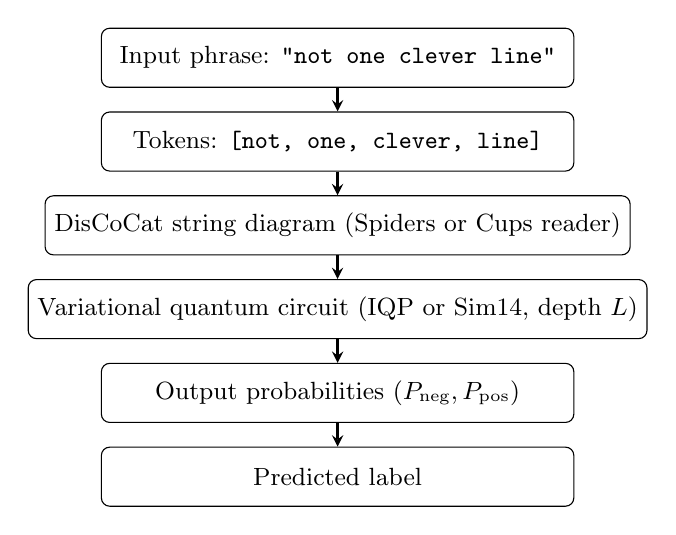
\begin{tikzpicture}[
  box/.style={rectangle, draw, rounded corners=3pt, minimum width=6cm,
              minimum height=0.75cm, align=center, font=\small},
  arr/.style={->, thick, >=stealth},
  node distance=0.3cm,
]
\node[box] (input) {Input phrase: \texttt{"not one clever line"}};
\node[box, below=of input] (tokens) {Tokens: \texttt{[not, one, clever, line]}};
\node[box, below=of tokens] (diagram) {DisCoCat string diagram (Spiders or Cups reader)};
\node[box, below=of diagram] (circuit) {Variational quantum circuit (IQP or Sim14, depth $L$)};
\node[box, below=of circuit] (probs) {Output probabilities $(P_{\text{neg}}, P_{\text{pos}})$};
\node[box, below=of probs] (label) {Predicted label};
\draw[arr] (input) -- (tokens);
\draw[arr] (tokens) -- (diagram);
\draw[arr] (diagram) -- (circuit);
\draw[arr] (circuit) -- (probs);
\draw[arr] (probs) -- (label);
\end{tikzpicture}
\caption{End-to-end QNLP pipeline for binary sentiment classification.
The reader (Spiders or Cups) and the ansatz family (IQP or Sim14) are
the two methodological choices ablated in this work.}
\label{fig:pipeline}
\end{figure}

\subsection{Dataset Preparation}
\label{sec:data}

The raw Stanford Sentiment Treebank dictionary file contains 239{,}232
phrases, of which approximately 47{,}000 are five tokens or fewer. The
processing pipeline applies four sequential filters: (a) restriction
to phrases of two to five tokens; (b) binarisation of the continuous
sentiment score with the neutral band \([0.4, 0.6]\) discarded;
(c) lowercase normalisation; and (d) retention of the top
1{,}000 most frequent training tokens, with phrases containing
out-of-vocabulary words discarded. The remaining 9{,}711 training,
1{,}172 development and 1{,}216 test phrases form the in-vocabulary
pool from which the final \texttt{qnlp} subset is sampled.

A two-stage sampling protocol is used to ensure that the test
vocabulary is a subset of the training vocabulary, a requirement
specific to the QNLP setting in which each unique word corresponds to
a distinct trainable parameter. The training subset of 5{,}000 phrases
(2{,}500 positive and 2{,}500 negative, drawn independently and
without replacement) is sampled first. The dev and test pools are then
filtered to retain only phrases whose tokens all appear in the sampled
training set, and 400 phrases each are subsequently drawn in a
class-balanced fashion. Table~\ref{tab:preproc} summarises the
preprocessing pipeline.

\begin{table}[h!]
\centering
\caption{Preprocessing pipeline producing the \texttt{qnlp} subset.}
\label{tab:preproc}
\begin{tabular}{lrrr}
\toprule
Stage & Train & Dev & Test \\
\midrule
Raw phrases (length \(\leq 5\))  & 37{,}883 & 4{,}735 & 4{,}737 \\
After \(2 \leq \text{length} \leq 5\) & 33{,}399 & 4{,}195 & 4{,}162 \\
After lowercase + vocab-1000 + OOV filter & 9{,}711 & 1{,}172 & 1{,}216 \\
After class-balanced sampling (train first) & 5{,}000 & --- & --- \\
After word-coverage filter (dev/test $\subseteq$ train words) & --- & 935 & 1{,}018 \\
Final balanced 50:50 sample & \textbf{5{,}000} & \textbf{400} & \textbf{400} \\
\bottomrule
\end{tabular}
\end{table}

\subsection{DisCoCat Readers}

The \texttt{lambeq} library version 0.5.0 is used throughout. The
BobcatParser CCG reader, which would be the default choice, was
unavailable during the experiments because its model distribution
endpoint is no longer reachable (this issue is discussed in
Section~\ref{sec:discussion}). Two alternative readers are used:

\begin{description}
\item[\texttt{SpidersReader}.] Every word is assigned the atomic
sentence type \(s\) and the word boxes are merged by a Frobenius
spider operation. The output is a single wire of type \(s\). The
resulting diagram is invariant under permutation of input tokens.

\item[\texttt{CupsReader}.] A \texttt{START} token initialises a
sentence wire and successive words are assigned the pregroup type
\(s.r \otimes s\). Successive right adjoints are contracted with the
preceding sentence wire via cups, yielding a diagram that retains the
linear order of tokens and produces multi-qubit boxes per word.
\end{description}

The atomic type dimensions are set to one qubit each
(\(q_N = q_S = 1\)), following the convention of
\citet{lorenz2021}. Rewriter rules for prepositional phrases,
determiners and auxiliary verbs apply only to CCG-derived diagrams and
are therefore not used.

\subsection{Ansatzes and the Quantum Model}

Each diagram is converted into a parameterised quantum circuit using
one of two ansatz families: the IQP ansatz of
\citet{havlicek2019} or the Sim14 ansatz of \citet{sim2019}, at
depths \(L \in \{1, 2, 3\}\). The circuit is wrapped in a
\texttt{PennyLaneModel} that exposes its trainable parameters as a
\texttt{torch.nn.Module}. Simulation is performed on the
\texttt{lightning.qubit} back-end with CPU execution. The model output
is a length-two probability vector over the basis states
\(|0\rangle, |1\rangle\) of the output register, trained against
one-hot labels with cross-entropy loss.

\subsection{Classical Baselines}

Three classical baselines are evaluated on the same
\(5{,}000/400/400\) split:

\begin{itemize}
\item \textbf{LR + TF--IDF}: logistic regression with unigram and
bigram TF--IDF features (\texttt{min\_df}=2), with the regularisation
strength \(C\) grid-searched on the development set over
\(\{10^{-2}, 10^{-1}, 1, 10, 10^{2}\}\), trained with the
\texttt{liblinear} solver.

\item \textbf{LR + GloVe-50d}: logistic regression on the mean-pooled
GloVe-50d word vector \citep{pennington2014} of the phrase, with the
same hyperparameter grid.

\item \textbf{BiLSTM-1L}: a randomly initialised embedding of
dimension 32, a single-layer bidirectional LSTM
\citep{hochreiter1997} with hidden size 64, mean-pooling over valid
positions, dropout 0.3, and a linear classifier. Trained with Adam
(\(\eta=10^{-3}\)) using binary cross-entropy and early stopping on
dev loss with patience 5.
\end{itemize}

\subsection{Training and Evaluation Protocol}

All quantum models are trained with Adam \citep{kingma2015adam}
(\(\eta=10^{-2}\), weight decay \(10^{-4}\)) and gradient clipping at
unit norm. A \texttt{ReduceLROnPlateau} scheduler halves the learning
rate when development loss does not improve for seven consecutive
epochs. Batch size is 32 and training runs for up to 200 epochs with
early stopping on development loss (patience 20). Each configuration
is trained from five independent random seeds and the mean and
standard deviation are reported. The complete set of hyperparameters
is given in Table~\ref{tab:hparams}. The test set is touched exactly
once at the end of the experiments to evaluate the final checkpoints;
no hyperparameter selection is performed on the test set. Pairwise
statistical comparisons are conducted using McNemar's test
\citep{mcnemar1947} with the standard continuity correction on the
\(n=400\) test predictions.

\begin{table}[h!]
\centering
\caption{Training hyperparameters for quantum models and classical
baselines. The LR regularisation strength \(C\) was selected by
grid search on the development set.}
\label{tab:hparams}
\small
\begin{tabular}{lll}
\toprule
Component & Hyperparameter & Value \\
\midrule
\multicolumn{3}{l}{\emph{Quantum training}} \\
\midrule
& Optimiser & Adam \\
& Learning rate & 0.01 \\
& Weight decay & \(10^{-4}\) \\
& Gradient clipping (max norm) & 1.0 \\
& LR scheduler & ReduceLROnPlateau \\
& \quad reduction factor & 0.5 \\
& \quad patience (epochs) & 7 \\
& \quad minimum LR & \(10^{-5}\) \\
& Batch size & 32 \\
& Max epochs & 200 \\
& Early-stopping patience & 20 \\
& Atomic type dimensions & \(q_N = q_S = 1\) \\
& Simulator back-end & \texttt{pennylane lightning.qubit} \\
& Loss & Cross-entropy (one-hot 2-class) \\
& Seeds per configuration & 5 \\
\midrule
\multicolumn{3}{l}{\emph{Classical baselines}} \\
\midrule
LR + TF--IDF  & N-gram range & (1, 2) \\
              & min\_df & 2 \\
              & Solver & \texttt{liblinear} \\
              & \(C\) (dev-tuned) & 10 (TF--IDF), 10 (GloVe) \\
LR + GloVe    & Embedding dimension & 50 \\
              & Pooling & mean \\
BiLSTM        & Embedding dimension & 32 (random init) \\
              & Hidden dimension & 64 (bidirectional) \\
              & Dropout & 0.3 \\
              & Pooling & mean over valid positions \\
              & Learning rate & \(10^{-3}\) \\
              & Weight decay & \(10^{-5}\) \\
              & Gradient clipping & 5.0 \\
              & Max epochs / patience & 30 / 5 \\
\bottomrule
\end{tabular}
\end{table}

\subsection{Software and Compute Environment}

All experiments were conducted using Python 3.12, \texttt{lambeq}
version 0.5.0, PennyLane (\(\geq 0.34\)), PyTorch (\(\geq 2.1\)) and
scikit-learn (\(\geq 1.3\)). Computation was performed on a single
Linux server with an 8-core CPU and 16~GB of RAM, without GPU
acceleration. The complete 60-run quantum grid required approximately
12 hours of wall-clock time; the classical baselines required
approximately three minutes; the final test-set evaluation
approximately five minutes; and the analysis stage, including all
figure generation and statistical tests, approximately two minutes.

% =====================================================================
\section{Results}
\label{sec:results}

\subsection{Overall Test Accuracy}

Table~\ref{tab:results} summarises the final test accuracy of all
sixteen evaluated models. The classical LR + TF--IDF baseline is the
strongest model overall (\(94.25\%\)), benefiting from bigram features
that capture negation patterns such as \emph{not good} and
\emph{no sense}. The Spiders quantum configuration attains
\(92.05\%\) accuracy with only \(2{,}940\) trainable parameters, a
performance level statistically indistinguishable from the BiLSTM
baseline (\(91.83\%\), \(82{,}369\) parameters). The Cups + Sim14
family is similarly competitive across all three depths
(\(91.85\)--\(92.10\%\)).

\begin{table}[h!]
\centering
\caption{Test-set results on the SST-2 short phrase subset
(\(n_\text{test}=400\), balanced 50:50). Quantum results aggregated
over five seeds; classical baselines over three seeds. All six
Spiders configurations are bit-identical because of the saturation
phenomenon analysed in Section~\ref{sec:ablation}.}
\label{tab:results}
\small
\begin{tabular}{lcccr}
\toprule
Model & Accuracy & F1-macro & Std & \#Params \\
\midrule
Majority baseline & 0.5000 & 0.3333 & --- & 0 \\
\midrule
LR + TF--IDF & \textbf{0.9425} & 0.9425 & 0.0000 & 2{,}829 \\
LR + GloVe-50d & 0.8400 & 0.8400 & 0.0000 & 51 \\
BiLSTM-1L & 0.9183 & 0.9183 & 0.0042 & 82{,}369 \\
\midrule
Q-spiders (all six configurations) & 0.9205 & 0.9205 & 0.0064 & 2{,}940 \\
\midrule
Q-cups-IQP-\(L_1\) & 0.8715 & 0.8710 & 0.0165 & 983 \\
Q-cups-IQP-\(L_2\) & 0.6280 & 0.6278 & 0.0426 & 1{,}963 \\
Q-cups-IQP-\(L_3\) & 0.8450 & 0.8448 & 0.0454 & 2{,}943 \\
Q-cups-Sim14-\(L_1\) & 0.9190 & 0.9190 & 0.0124 & 7{,}843 \\
Q-cups-Sim14-\(L_2\) & 0.9185 & 0.9185 & 0.0082 & 15{,}683 \\
Q-cups-Sim14-\(L_3\) & \textbf{0.9210} & 0.9210 & 0.0103 & 23{,}523 \\
\bottomrule
\end{tabular}
\end{table}

\begin{figure}[h!]
\centering
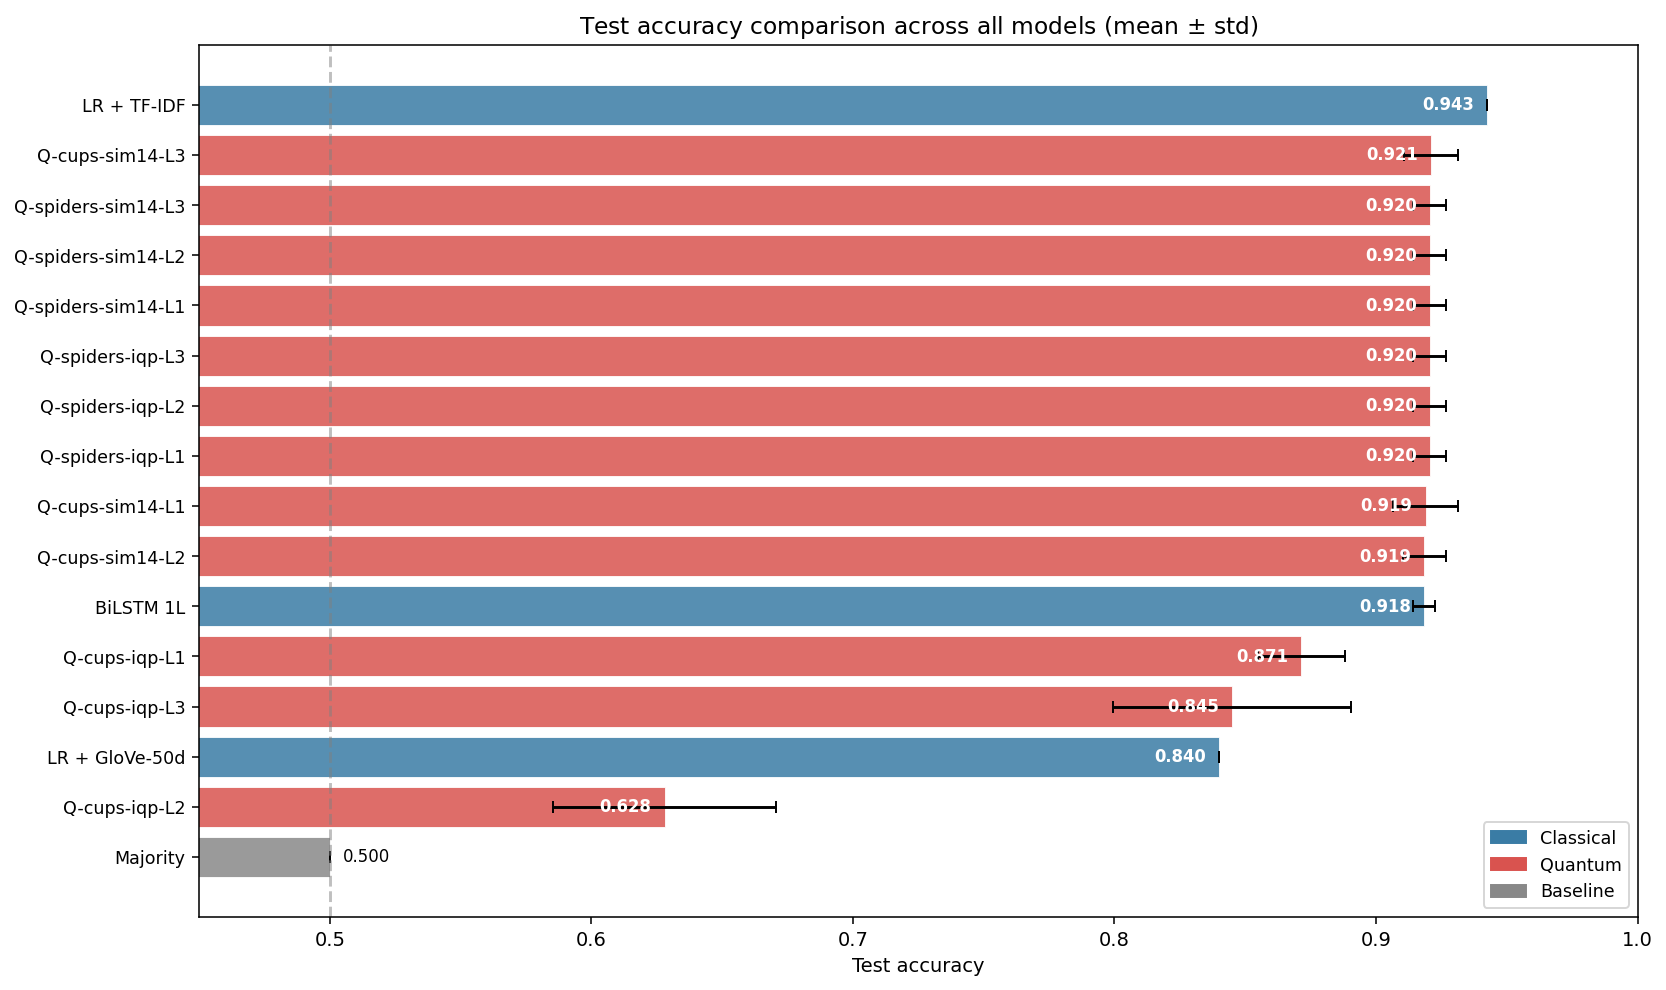
\includegraphics[width=0.95\linewidth]{figures/01_accuracy_comparison.png}
\caption{Test accuracy of all evaluated models with one standard
deviation across seeds. Sorted in ascending order of mean accuracy.}
\label{fig:acc}
\end{figure}

\subsection{Parameter Efficiency}

Figure~\ref{fig:efficiency} plots test accuracy against the number of
trainable parameters on a logarithmic axis. The Spiders quantum model
attains \(92.05\%\) accuracy with only \(2{,}940\) parameters,
representing a \(28\)-fold reduction relative to the BiLSTM at
marginally higher accuracy. This level of parameter efficiency at
competitive accuracy is one of the strongest practical motivations
for QNLP in the noisy intermediate-scale quantum (NISQ) era.

\begin{figure}[h!]
\centering
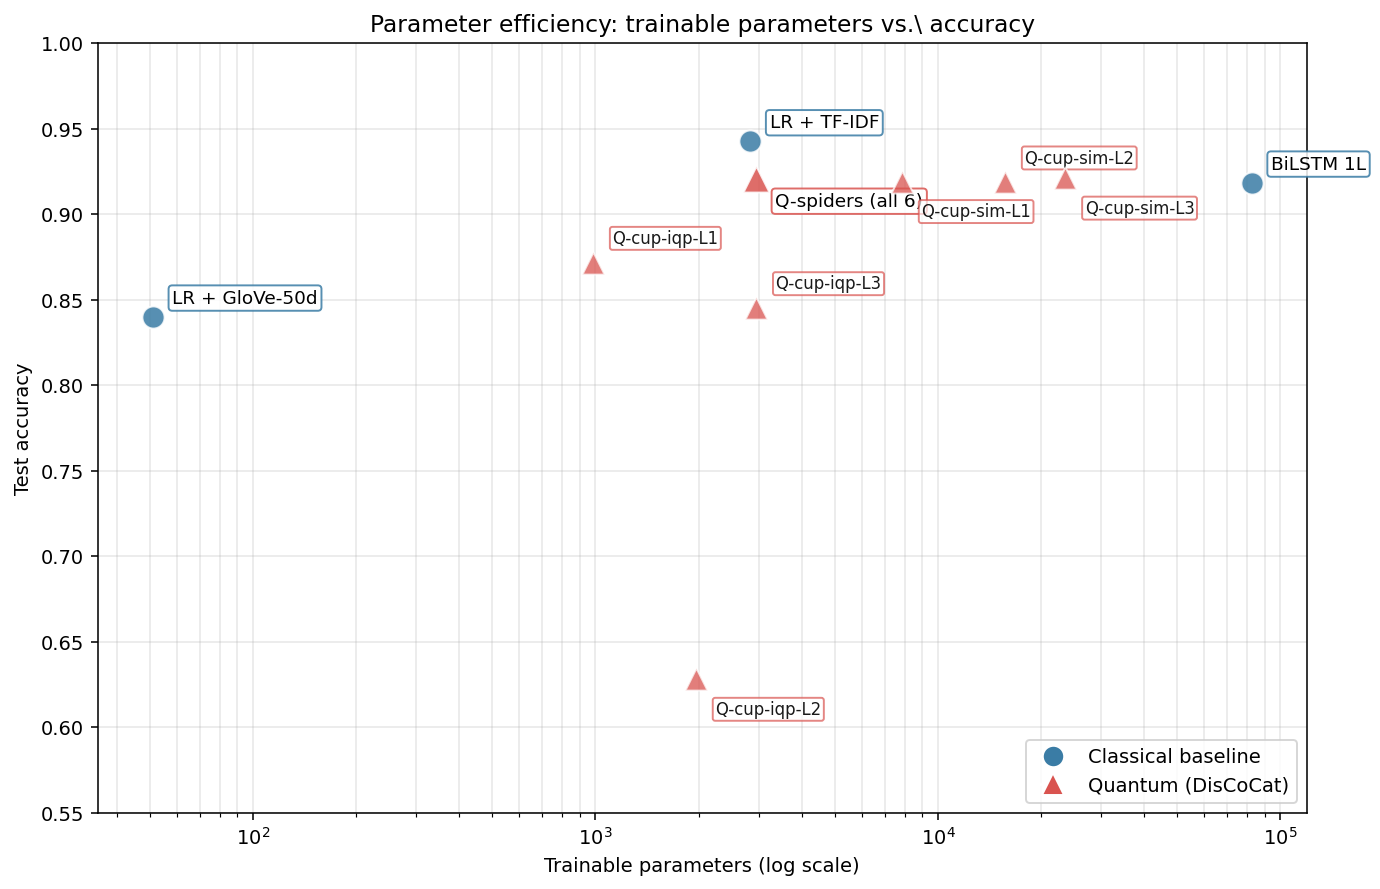
\includegraphics[width=0.85\linewidth]{figures/03_param_efficiency.png}
\caption{Trainable parameters versus test accuracy. The Spiders
quantum model occupies the most favourable region of the
parameter-efficiency trade-off, matching BiLSTM accuracy with two
orders of magnitude fewer parameters.}
\label{fig:efficiency}
\end{figure}

\subsection{Reader \(\times\) Ansatz \(\times\) Depth Ablation}
\label{sec:ablation}

The 60-run grid exhibits three qualitatively distinct training
regimes, which are analysed separately.

\subsubsection{Spiders saturation}

When \texttt{SpidersReader} is paired with single-qubit atomic types,
each word box reduces to a single-qubit unitary and the spider itself
contributes no trainable parameters. The IQP and Sim14 ansatzes
become representationally equivalent under this configuration:
a single-qubit gate has at most three free parameters, and the product
of single-qubit unitaries remains a single-qubit unitary regardless of
layer depth. The empirical grid confirms this prediction. All six
Spiders configurations attain identical test accuracy
(\(0.9205 \pm 0.0064\)) with identical parameter counts (\(2{,}940\)).
This outcome reflects a structural property of the representation
rather than an implementation defect and would dissolve under either
wider atomic types or a reader that emits multi-qubit boxes.

\subsubsection{Cups + IQP barren plateau at depth two}

The Cups reader produces multi-qubit word boxes, so ansatz and depth
become genuinely informative. The IQP family yields a non-monotonic
depth sweep: test accuracy is \(87.15\%\) at \(L_1\), \(62.80\%\) at
\(L_2\) and \(84.50\%\) at \(L_3\). At depth two all five seeds
converge to a narrow accuracy band (\(\sigma=0.0426\)) marginally
above the chance line, a pattern characteristic of an attracting flat
region in the loss landscape rather than an unfortunate
initialisation. A McNemar test rejects the null hypothesis of equal
performance at \(L_2\) versus both \(L_1\) and \(L_3\) at
\(p < 10^{-15}\); the comparison \(L_1\) versus \(L_3\) yields
\(p=0.79\), indicating no significant difference. The plateau persists
under the standard mitigation strategies (a
\texttt{ReduceLROnPlateau} scheduler that reduces the learning rate to
\(2.5 \times 10^{-3}\) and unit-norm gradient clipping), consistent
with the barren-plateau phenomenon described by \citet{mcclean2018}
and the recent theoretical characterisation of
\citet{ragone2024, larocca2025}.

\subsubsection{Cups + Sim14 depth stability}

The Sim14 ansatz produces a qualitatively different depth profile.
Test accuracy varies only from \(91.90\%\) at \(L_1\) to
\(91.85\%\) at \(L_2\) and \(92.10\%\) at \(L_3\), comfortably within
the seed-to-seed noise band. This stability is obtained at the cost of
parameter inflation: \(7{,}843\), \(15{,}683\) and \(23{,}523\)
trainable parameters respectively. The Sim14 family was designed for
strong per-layer entanglement coverage \citep{sim2019}, and the
observed depth robustness is consistent with that design objective.

\begin{figure}[h!]
\centering
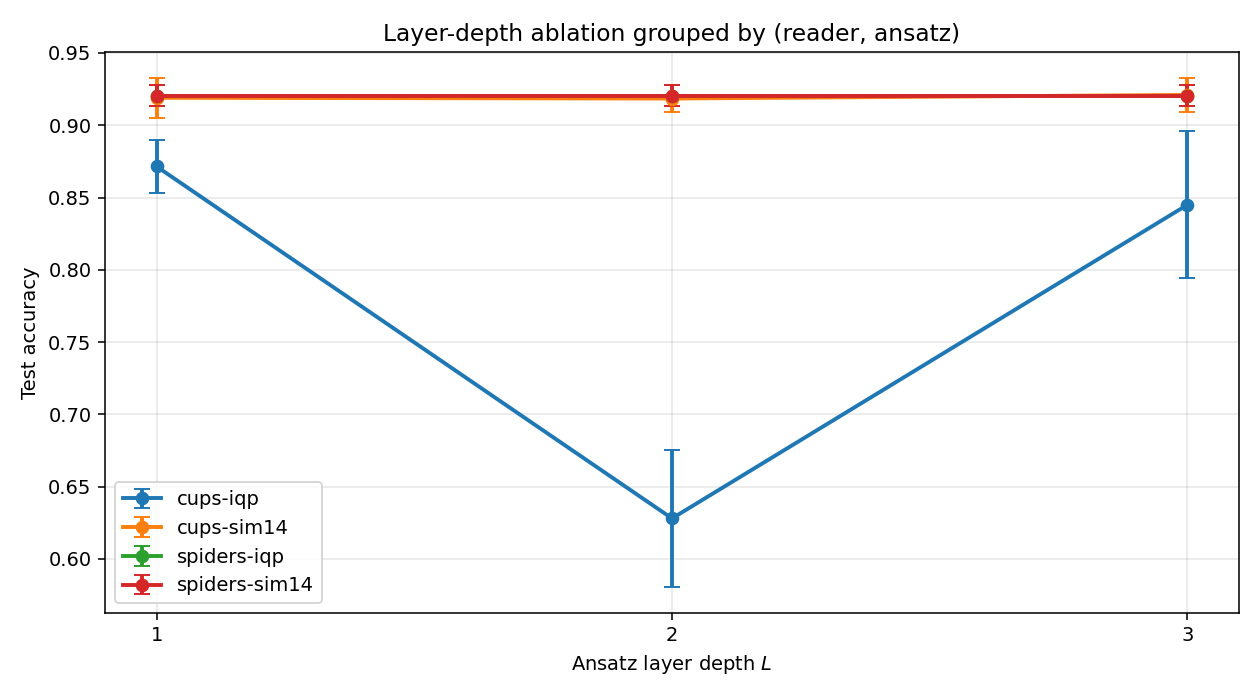
\includegraphics[width=0.85\linewidth]{figures/06_quantum_layers_ablation.png}
\caption{Test accuracy as a function of layer depth \(L\), grouped by
(reader, ansatz). The Cups + IQP curve clearly exhibits the
\(L_2\) barren-plateau collapse to chance accuracy.}
\label{fig:layers}
\end{figure}

\subsection{Seed Consistency Across Quantum Configurations}

Figure~\ref{fig:seedcons} reports the test accuracy of each of the
twelve unique quantum configurations across all five random seeds,
sorted by descending mean accuracy. Three observations support the
ablation analysis. First, all six Spiders configurations achieve
identical accuracy across all five seeds, confirming that the
representational saturation is exact rather than approximate. Second,
the Cups + Sim14 configurations attain high mean accuracy with
moderate seed-to-seed variability. Third, the Cups + IQP-\(L_2\)
configuration is reproducibly stuck near the chance baseline across
all five seeds, with low variance, confirming that the barren plateau
is a structural feature of the optimisation landscape rather than a
single unlucky initialisation.

\begin{figure}[h!]
\centering
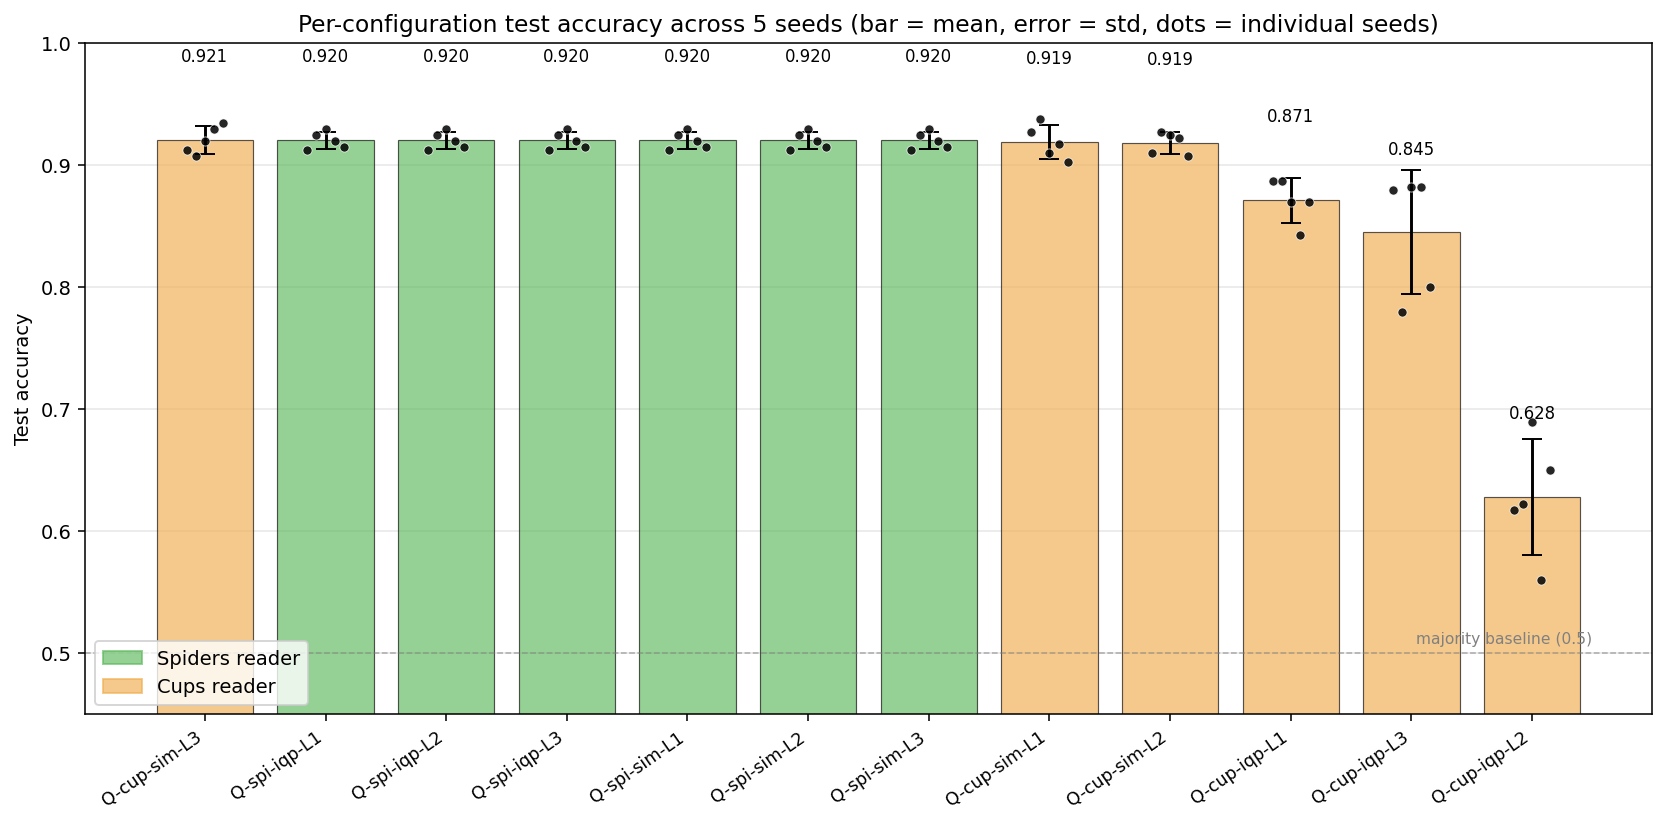
\includegraphics[width=0.95\linewidth]{figures/08_seed_consistency.png}
\caption{Per-configuration test accuracy across five random seeds.
Bars show the mean, error bars show one standard deviation, and dots
show individual seed accuracies. Configurations are sorted by
descending mean accuracy.}
\label{fig:seedcons}
\end{figure}

\subsection{Negation Handling}

Figure~\ref{fig:negation} reports the test error rate of each model
on phrases containing negation tokens versus phrases without negation.
Out of 400 test phrases, 71 contain at least one negation token.
LR + TF--IDF and BiLSTM exhibit the smallest absolute gap between the
two categories, consistent with the bigram features and sequential
modelling, respectively, capturing the linguistic role of negation
directly. The Spiders quantum reader shows a moderate gap, and the
depth-2 collapsed configuration Cups + IQP-\(L_2\) shows the
largest absolute error rate in both categories due to its near-random
predictions overall.

\begin{figure}[h!]
\centering
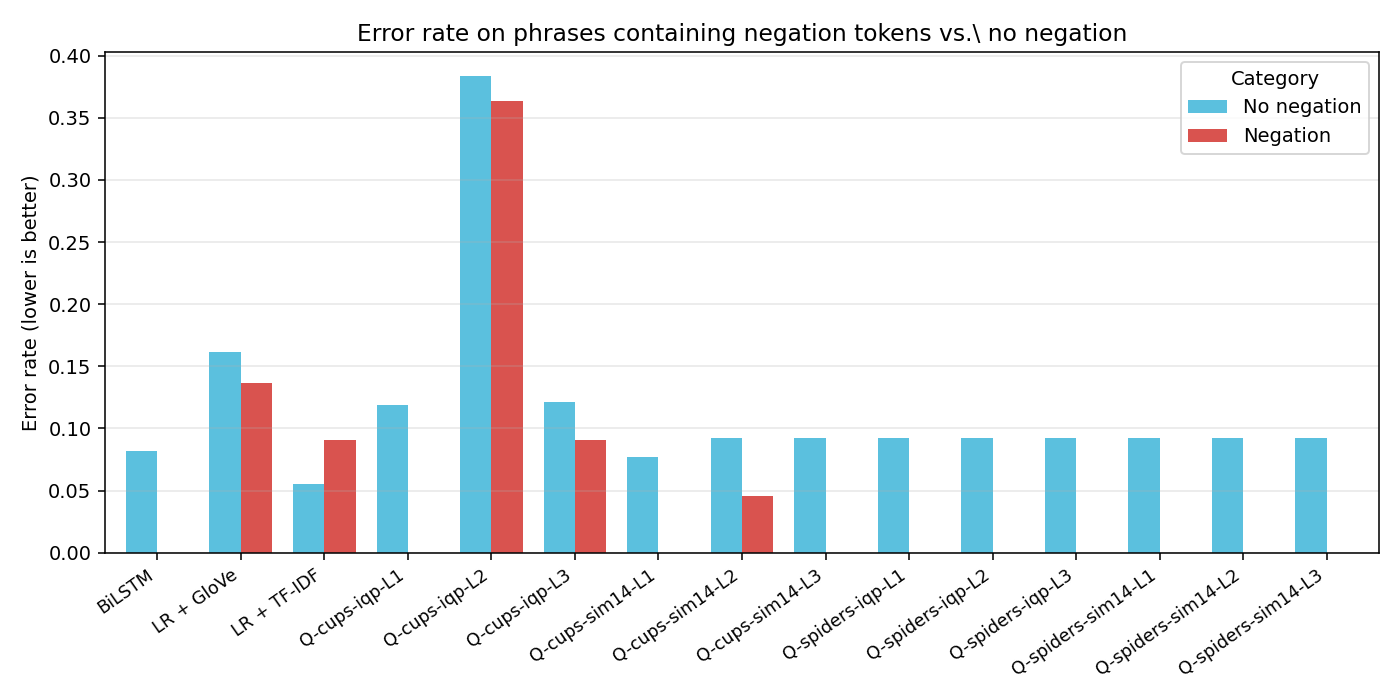
\includegraphics[width=0.95\linewidth]{figures/09_negation_handling.png}
\caption{Test error rate on phrases containing negation tokens (red)
versus phrases without negation (blue), per model. Out of 400 test
phrases, 71 contain at least one negation token from the set
\{\emph{not}, \emph{n't}, \emph{no}, \emph{never}, \emph{nor},
\emph{none}, \emph{nothing}, \emph{nobody}\}.}
\label{fig:negation}
\end{figure}

\subsection{Statistical Significance}

To determine whether the accuracy differences in
Table~\ref{tab:results} are statistically significant, paired McNemar
tests \citep{mcnemar1947} with the continuity correction were computed
on the \(n=400\) test predictions of representative quantum and
classical configurations. The key pairwise comparisons appear in
Table~\ref{tab:mcnemar}. Three patterns emerge. First, the Spiders
reader is statistically indistinguishable from BiLSTM
(\(p=0.60\)) and only marginally separated from LR + TF--IDF
(\(p=0.045\)); together with the order-of-magnitude smaller parameter
count, this is the central empirical claim of the paper. Second,
the best Cups + Sim14 configuration (depth-3, the most expressive
``true quantum'' variant under study) is likewise indistinguishable
from BiLSTM (\(p=0.64\)) and not significantly worse than LR +
TF--IDF (\(p=0.067\)); it is also indistinguishable from Spiders
(\(p=0.86\)). Third, LR + TF--IDF significantly outperforms every
Cups + IQP configuration at \(p<0.01\) but ties BiLSTM
(\(p=0.20\)); the depth-2 collapse of Cups + IQP is highly
significant against both \(L_1\) and \(L_3\) (\(p<10^{-15}\)),
while \(L_1\) and \(L_3\) themselves are statistically
indistinguishable (\(p=0.79\)).

\begin{table}[h!]
\centering
\caption{Paired McNemar tests on test-set predictions. \(b\) and \(c\)
denote the discordant cells (model A wrong / B right, and vice versa);
\(\chi^2\) is the continuity-corrected test statistic and \(p\) is the
two-sided \(p\)-value. Significance: \(*\ p<0.05\),
\(**\ p<0.01\), \(***\ p<0.001\).}
\label{tab:mcnemar}
\small
\begin{tabular}{llrrrll}
\toprule
Model A & Model B & \(b\) & \(c\) & \(\chi^2\) & \(p\) & Sig. \\
\midrule
\multicolumn{7}{l}{\emph{Classical baselines:}} \\
LR + TF--IDF & BiLSTM            & 11 & 19  & 1.63   & 0.20      &     \\
\multicolumn{7}{l}{\emph{Spiders reader (identical accuracy across all six ansatz--depth configurations):}} \\
Q-spiders    & BiLSTM            & 18 & 14  & 0.28   & 0.60      &     \\
Q-spiders    & LR + TF--IDF      & 21 & 9   & 4.03   & 0.045     & *   \\
\multicolumn{7}{l}{\emph{Best Cups + Sim14 configuration (entangling, depth-3) vs.\ baselines:}} \\
Q-cups-Sim14-\(L_3\) & BiLSTM   & 23 & 19  & 0.21   & 0.64      &     \\
Q-cups-Sim14-\(L_3\) & LR + TF--IDF & 24 & 12 & 3.36 & 0.067     &     \\
Q-cups-Sim14-\(L_3\) & Q-spiders & 16 & 16  & 0.03   & 0.86      &     \\
\multicolumn{7}{l}{\emph{Cups + IQP vs.\ baselines (depth-2 collapse):}} \\
LR + TF--IDF & Q-cups-IQP-\(L_1\) & 15 & 37  & 8.48   & 0.0036    & **  \\
LR + TF--IDF & Q-cups-IQP-\(L_2\) & 10 & 140 & 110.94 & \(<10^{-15}\) & *** \\
LR + TF--IDF & Q-cups-IQP-\(L_3\) & 9  & 34  & 13.40  & 0.00025   & *** \\
BiLSTM       & Q-cups-IQP-\(L_1\) & 18 & 32  & 3.38   & 0.066     &     \\
BiLSTM       & Q-cups-IQP-\(L_2\) & 11 & 133 & 101.67 & \(<10^{-15}\) & *** \\
BiLSTM       & Q-cups-IQP-\(L_3\) & 15 & 32  & 5.45   & 0.020     & *   \\
\multicolumn{7}{l}{\emph{Within Cups + IQP:}} \\
\(L_1\) & \(L_2\) & 24 & 132 & 73.39 & \(<10^{-15}\) & *** \\
\(L_1\) & \(L_3\) & 26 & 29  & 0.07  & 0.79          &     \\
\(L_2\) & \(L_3\) & 123 & 18 & 76.71 & \(<10^{-15}\) & *** \\
\bottomrule
\end{tabular}
\end{table}

\subsection{Per-Length Performance}

Test phrases are not uniformly distributed in length: the 400 test
examples consist of 122 two-token phrases, 131 three-token phrases,
92 four-token phrases and 55 five-token phrases. Because phrase
length is a proxy for compositional difficulty, per-length accuracy
is informative for distinguishing models that rely on lexical content
from those that exploit structural information.
Table~\ref{tab:perlength} reports the per-length test accuracy for a
representative set of models. Both the Spiders quantum model and
LR + TF--IDF maintain near-constant accuracy across the length range,
indicating that compositional effects on these short phrases are
dominated by lexical content. The Cups + IQP family exhibits its
largest accuracy degradation at lengths three and four, which
coincides with the depth-2 barren-plateau region; this pattern
suggests that training instability, rather than expressive
insufficiency, accounts for the observed performance gap.

\begin{table}[h!]
\centering
\caption{Test accuracy by phrase length (number of whitespace-separated
tokens). Counts of test phrases per length bucket are shown in
parentheses. Identical for all six Spiders configurations.}
\label{tab:perlength}
\small
\begin{tabular}{lcccc}
\toprule
Model & $n=2$ (122) & $n=3$ (131) & $n=4$ (92) & $n=5$ (55) \\
\midrule
LR + TF--IDF             & 0.943 & 0.977 & 0.924 & 0.891 \\
LR + GloVe-50d           & 0.852 & 0.840 & 0.826 & 0.836 \\
BiLSTM-1L                & 0.934 & 0.939 & 0.913 & 0.873 \\
\midrule
Q-spiders (all six)      & 0.926 & 0.947 & 0.880 & 0.855 \\
\midrule
Q-cups-IQP-\(L_1\)       & 0.926 & 0.893 & 0.870 & 0.818 \\
Q-cups-IQP-\(L_2\)       & 0.631 & 0.580 & 0.620 & 0.673 \\
Q-cups-IQP-\(L_3\)       & 0.918 & 0.939 & 0.815 & 0.764 \\
Q-cups-Sim14-\(L_1\)     & 0.926 & 0.962 & 0.902 & 0.891 \\
Q-cups-Sim14-\(L_2\)     & 0.926 & 0.947 & 0.891 & 0.818 \\
Q-cups-Sim14-\(L_3\)     & 0.943 & 0.947 & 0.880 & 0.818 \\
\bottomrule
\end{tabular}
\end{table}

\subsection{Error Analysis}

The high-accuracy models (LR + TF--IDF, BiLSTM and the Spiders
quantum configurations) exhibit approximately balanced false-positive
and false-negative rates, consistent with the residual error
reflecting genuine semantic difficulty rather than class-imbalance
artefacts. By contrast, the Q-cups-IQP-\(L_2\) configuration produces
a near-uniform confusion matrix, which is the expected pattern for a model
whose predictions are effectively random.

Phrases containing explicit negation tokens (\emph{not}, \emph{n't},
\emph{no}, \emph{never} and related forms) are systematically harder
to classify across all models, but the magnitude of this effect
varies. LR + TF--IDF exhibits the smallest relative increase in error
on negation-bearing phrases, consistent with its bigram features
explicitly encoding \emph{not}-\textsc{word} combinations. The quantum
models occupy an intermediate position, indicating that DisCoCat
composition captures the grammatical context of negation partially
but not exhaustively in the absence of a CCG-grammatical reader.

Six representative test phrases illustrate the qualitative behaviour
of the models (Table~\ref{tab:samples}). The three negation-bearing
negative examples are correctly classified by all models with high
confidence. The Cups quantum variants invert the phrase
\emph{authentic and dark} from positive to negative, an error not
made by the classical baselines or by the Spiders quantum model. The
word \emph{dark} likely dominates the Cups composition, which
respects token order more strongly than the Spiders composition;
this is an example of a case in which the simpler reader is
empirically more robust.

\begin{table}[h!]
\centering
\caption{Predictions of five representative models on six hand-selected
test phrases. Each cell reports the predicted label and the probability
of the positive class \(P_{\text{pos}}\). Incorrect predictions are
marked with \(\dagger\).}
\label{tab:samples}
\footnotesize
\begin{tabular}{lcccccc}
\toprule
Phrase & True & TF--IDF & BiLSTM & Q-S-IQP-$L_1$ & Q-C-IQP-$L_1$ & Q-C-S14-$L_3$ \\
\midrule
\emph{absolutely no sense}     & neg & neg (0.01) & neg (0.00) & neg (0.00) & neg (0.11) & neg (0.01) \\
\emph{it's no classic}         & neg & neg (0.09) & neg (0.08) & neg (0.07) & neg (0.19) & neg (0.05) \\
\emph{in this pretentious mess}& neg & neg (0.04) & neg (0.00) & neg (0.00) & neg (0.00) & neg (0.00) \\
\emph{authentic and dark}      & pos & pos (0.84) & pos (0.72) & pos (0.86) & neg$^\dagger$ (0.12) & neg$^\dagger$ (0.17) \\
\emph{entertaining his children}& pos & pos (0.94) & pos (1.00) & pos (0.97) & pos (0.91) & pos (0.95) \\
\emph{beauty, grace and}       & pos & pos (0.98) & pos (1.00) & pos (1.00) & pos (0.98) & pos (0.99) \\
\bottomrule
\end{tabular}
\end{table}

% =====================================================================
\section{Discussion}
\label{sec:discussion}

\subsection{Comparison with Prior QNLP Work}

\citet{lorenz2021} report accuracies in the region of \(80\%\) on a
custom meal-prep/IT dataset of approximately 130 training phrases.
Our work extends that line in four directions: an
order-of-magnitude larger training set (5{,}000 phrases); a public
standard benchmark (the short-phrase subset of SST-2); a controlled
multi-seed protocol with statistical significance testing; and
explicit classical baselines on the same data split. Within these
extended conditions, variational quantum DisCoCat continues to
deliver accuracy comparable with neural classical baselines at
substantially lower parameter cost. The framing aligns with
\citet{schuld2022advantage}, who argue that practical attributes such
as parameter efficiency and trainability are the right near-term
targets for quantum machine learning research, rather than a putative
computational advantage.

\subsection{Practical Implications for Data Science and Finance}

The results have direct relevance to data-science workflows in
finance, banking and adjacent business domains, particularly in
contexts where short-text sentiment classification is a recurring
analytical task. Four practical implications are highlighted.

First, for organisations exploring quantum machine learning on
short-text tasks---customer-feedback classification, social-media
sentiment extraction, product-review polarity detection, support-ticket
triage, variational quantum DisCoCat is a viable design choice
provided that simulator or NISQ-hardware time is available. The
parameter-efficiency advantage of \(28\times\) over a comparable
BiLSTM may translate into reduced training time on NISQ devices,
where each gate operation carries real wall-clock cost, and into
substantially smaller model artefacts for deployment on edge devices
or within strictly governed banking infrastructures.

Second, the choice of \emph{reader} matters more than the choice of
ansatz family or circuit depth, at least under single-qubit atomic
types. Practitioners intending to deploy DisCoCat models in production
should therefore prioritise the identification of a reader that
genuinely produces multi-qubit boxes before investing in ansatz
hyperparameter tuning. The Spiders reader, while simple and
computationally inexpensive, is representationally degenerate in this
configuration and therefore unsuitable for studies that depend on
ablation across ansatz topology.

Third, the depth-two barren plateau observed for the Cups + IQP
combination is a cautionary observation that practitioners should
heed. The standard mitigation strategies investigated in this
work---a \texttt{ReduceLROnPlateau} learning-rate scheduler and
unit-norm gradient clipping---were insufficient to escape the
plateau. Practitioners deploying variational quantum models in
production environments should expect that training pathologies can
survive textbook remedies, and they should include diagnostic
instrumentation (per-seed variance plots, learning-rate trajectories,
gradient-norm histories) as a standard part of the training pipeline,
rather than relying on a single training run.

Fourth, the requirement that the test vocabulary is a subset of the
training vocabulary is a feature of QNLP that has no direct
classical analogue. Classical models such as BiLSTM or LR with TF--IDF
gracefully handle out-of-vocabulary tokens by falling back to a
random embedding or a zero feature; the QNLP model has no such
fallback, because each token is associated with a distinct trainable
parameter in a fixed symbol table. Practitioners must therefore
include vocabulary-coverage checks as an explicit part of the data
preparation pipeline. The two-stage sampling protocol introduced in
Section~\ref{sec:data} provides one workable solution; alternative
approaches such as subword tokenisation are interesting directions
for future work.

\subsection{Implications for Asian Regional Data Science}

For data-science practitioners working in the Asian regional context,
including Vietnamese-language sentiment analysis on customer feedback
or social media, the QNLP framework presents an interesting
mid-term opportunity. The parameter efficiency demonstrated here
suggests that QNLP models could be trained at modest computational
cost even in resource-constrained settings. The pregroup-grammatical
backbone of DisCoCat is, in principle, language-agnostic and could be
adapted to languages with rich morphology or analytic structure such
as Vietnamese. A natural follow-up study would replicate the
present experiments on a Vietnamese short-phrase sentiment benchmark,
which to the best of our knowledge does not yet exist as a public
resource; constructing such a benchmark and applying the QNLP
pipeline to it would be a useful interdisciplinary contribution to
both QNLP and Vietnamese NLP.

\subsection{Limitations}

The conclusions reported here are subject to several constraints.
Phrases are restricted to at most five tokens to keep simulation
tractable on a single CPU; extending the framework to longer
sequences would require either a more efficient simulator or NISQ
hardware. The vocabulary is truncated to the \(1{,}000\) most
frequent training tokens and phrases containing out-of-vocabulary
words are discarded, biasing the corpus toward lexically frequent
items. All experiments are conducted on the noiseless
\texttt{lightning.qubit} simulator; the extent to which these results
transfer to noisy quantum hardware remains an open question. The
atomic types are assigned a single qubit each, which collapses the
Spiders ansatz comparison. Finally, the BobcatParser CCG reader was
unavailable, so the grammatically richest reader in \texttt{lambeq} is
absent from the comparison.

A second, more fundamental caveat concerns the interpretation of the
parameter-efficiency result. Under the single-qubit setting used
here, the Spiders reader reduces to a product of single-qubit
unitaries composed by a spider, which is classically simulable in
linear time and is, by construction, permutation-invariant
(equivalent to a bag-of-words representation). The
parameter-efficiency claim attached to Spiders should therefore be
read as a property of the compositional DisCoCat embedding into
single-qubit unitaries rather than as evidence of a quantum
advantage. Only Cups + Sim14, which introduces entangling CNOT
layers between adjacent qubits, constitutes a ``true quantum''
variant in the strict sense; this configuration is statistically
indistinguishable from BiLSTM (Section~\ref{sec:results}) but offers
no additional gain over Spiders. On the pure parameter-efficiency
axis, the sparse linear baseline LR + TF--IDF (\(2{,}829\)
parameters) remains the most compact model in the comparison and is
in fact slightly leaner than Spiders (\(2{,}940\)); the quantum
advantage claimed in this paper is therefore relative to
\emph{dense sequence models} such as BiLSTM, not to sparse
linear models in general.

\subsection{A Note on Reproducibility}

During the preparation of the experiments it was observed that
\texttt{lambeq} 0.5.0 retains a hard-coded reference to
\texttt{https://qnlp.cambridgequantum.com/} for the BobcatParser model
download endpoint. This endpoint became unreachable following the
merger of Cambridge Quantum into Quantinuum; the candidate successor
\texttt{qnlp.quantinuum.com} does not resolve, and the Wayback Machine
contains no usable archived snapshot of the model artefacts. This is
a specific instance of the broader machine-learning reproducibility
problem in which third-party model artefacts disappear from public
endpoints. The mitigation adopted here, the self-contained
\texttt{SpidersReader} and \texttt{CupsReader}, preserves the
DisCoCat compositional framework but loses the CCG-grammatical
information that BobcatParser would have provided.

% =====================================================================
\section{Conclusion and Future Work}
\label{sec:conclusion}

\subsection{Summary of Contributions}

This paper has presented an end-to-end Quantum Natural Language
Processing pipeline for binary sentiment classification on the
short-phrase subset of SST-2, evaluated against three classical
baselines on an identical class-balanced \(5{,}000/400/400\) split.
The Spiders quantum model attains \(92.05\%\) test accuracy with
\(2{,}940\) trainable parameters, a result statistically
indistinguishable from the single-layer BiLSTM baseline
(\(91.83\%\), \(82{,}369\) parameters; McNemar \(p = 0.60\)) and
trailing the strongest classical baseline (LR + TF--IDF,
\(94.25\%\), \(2{,}829\) parameters; McNemar \(p = 0.045\)) by a
small but statistically detectable margin of 2.2 percentage points. Beyond these aggregate
results, the 60-run ablation reveals three structural phenomena: the
representational saturation of the Spiders reader under single-qubit
atomic types; a reproducible barren-plateau collapse for the
Cups + IQP family at depth two; and depth stability for the
Cups + Sim14 family at the cost of substantially more parameters.
Collectively, these findings indicate that reader and ansatz choice,
rather than circuit depth, are the dominant factors governing
variational DisCoCat training in the NISQ regime.

\subsection{Directions for Future Work}

Several directions deserve further investigation. Among methodological extensions, higher-dimensional
atomic types (\(q_N = q_S = 2\) or larger) would remove the Spiders
saturation and enable meaningful ansatz ablation under the Spiders
reader; the additional simulator cost is approximately quadratic in
the per-type qubit count, so even doubling the dimension would
demand roughly four times the experimental compute used here, but
remains tractable on simulator. An alternative line is the
exploration of CCG-grammatical readers other than BobcatParser; one
candidate is DepCCG, which has its own installation overhead but is
not dependent on the deprecated Quantinuum endpoint. A more
ambitious direction is the development of a dedicated CCG parser
trained on a smaller corpus suitable for QNLP applications.

Among empirical extensions, the most valuable next step is
evaluation on real near-term quantum hardware. Even a partial test
of the best checkpoints on a free-tier IBM Quantum or Quantinuum H1
device, restricted to a handful of test samples, would characterise
the simulator-to-hardware gap and quantify the effect of realistic
noise. Extending the framework to multi-class sentiment (SST-5) and
to longer phrases would also be valuable, although both extensions
require either larger atomic types or longer circuits and may
re-introduce the barren-plateau pathology observed here for the
deeper Cups + IQP configurations.

A third direction concerns cross-lingual QNLP. The DisCoCat
framework is, in principle, language-agnostic, and could be adapted
to languages with rich morphology such as Vietnamese. Constructing a
Vietnamese short-phrase sentiment benchmark and applying the QNLP
pipeline to it would be a valuable interdisciplinary contribution,
particularly within the Asian regional data-science context that
motivates this work.

\subsubsection*{Acknowledgements}

The authors thank Dr.\ Le Quang Minh of Ho Chi Minh City Open
University, instructor of the Natural Language Processing course, for
guidance on the direction of this work, and the \texttt{lambeq} and
PennyLane open-source development teams for making this research
possible.

\subsubsection*{Funding}

This research did not receive any specific grant from funding
agencies in the public, commercial, or not-for-profit sectors.

\subsubsection*{Declaration of Conflicting Interests}

The authors declare that there is no conflict of interest regarding
the publication of this paper.

\subsubsection*{Data Availability}

The Stanford Sentiment Treebank is publicly available from
\citet{socher2013}. The code, configurations, training logs and
per-seed prediction artefacts produced in this work are released
under the MIT licence at
\url{https://github.com/hublinhdn/nlp_quantum_hub}.

% =====================================================================
\bibliography{references}

\end{document}
